%%% 第三章 机械臂抓取系统实现
%%%%%%%%%%%%%%%%%%%%%%%%%%%%%%%%
\chapter{图像处理模块设计与实现}
图像处理模块是自动分拣系统中的核心模块,关系着整个系统的性能表现。图像处理模块相当于自动分拣系统的“大脑”,
其中目标检测算法的预测用时将直接影响自动分拣系统的实时性,目标检测算法的准确率将直接影响自动分拣系统的分拣
准确率。因此,自动分拣系统的图像处理模块需要进行深入地研究和设计。本课题设计的自动分拣系统中的图像处理模块
使用了基于深度学习的目标检测算法和传统的计算图像相似度的图像算法,以便最大幅度提升图像处理模块的实时性,降低
系统延时。

本章主要介绍课题所设计的自动分拣系统中的图像处理模块,包括目标检测算法输入之前的图像预处理、基于深度学习的
目标检测算法的理论及其实际训练评估过程。最后介绍了如何将训练好的深度学习模型部署到Jetson TX2上,将其封装为
ROS节点,接入系统的通信网络。

\section{图像算法理论}
目标检测是计算机视觉领域的计算机技术,其涉及在数字图像和视频中检测特定对象的实例。目标检测算法应用十分广泛,
如人脸检测、人脸识别、对象跟踪等,当然,还有本论文中的工件识别。

基于深度学习的目标检测算法具有可移植性强、效果优异的优点,但深度学习模型一般具有海量的网络参数,
计算量大,运算效率不高。而自动分拣系统的场景下,并不是每一帧图像都需要输入目标检测算法进行工件
位置和类别的预测。一般情况下,只需要在机械臂执行之前进行预测。因此,本课题的图像处理模块,在图像信息
输入目标检测算法节点之前,加入了一个图像预处理节点,用于接收摄像头发送的图像信息,进行简单计算,判断
是否将该图像信息发送到目标检测算法节点。

本节将介绍课题中使用的两种图像算法:感知哈希算法\cite{ganzhihash}和YOLOv3。其中感知哈希算法用于图象预处理节点,用于判断工件是否处于
可抓取状态,若可抓取,则将图像发送到运行目标检测算法的节点进行处理,否则不进行处理。YOLOv3算法用于识别图像中
工件的位置和类别,为抓取提供信息。

\subsection{感知哈希算法}

自动分拣系统的场景中,我们希望机械臂抓取之前才进行目标检测步骤,以降低系统计算量,降低系统延时。本课题设计的自动分拣
系统,在工件静止时进行抓取,因此使用感知哈希算法来判断工件是否已经静止。感知哈希算法本身是用于图片相似度计算的算法,
可以通过计算前后几帧图片的相似度来间接判断图片是否静止。

感知哈希算法对每张图片生成一个“指纹”字符串,然后比较不同图片的指纹。结果越相近,说明图片越相似。其算法实现步骤如下:
\begin{enumerate}
    \item{第一步,缩小尺寸。
    
    将图片缩小到8×8的尺寸共64个像素点。这一步的目的是去除图片细节,只保留结构、明暗等基本信息。}
    \item{第二步,简化色彩。
    
    将第一步得到的图片,转化为64级灰度。即所有像素点只有64种灰度颜色。}
    \item{第三步,计算平均值。
    
    计算第二步得到的灰度图像的像素点平均值。}
    \item{第四步,比较像素灰度。
    
    将第二步得到的灰度图像中的像素点逐个与平均值比较,大于或等于平均值记为1,否则记为0。}
    \item{第五步,计算哈希值。
    
    将第四步的结果组合在一起得到一个64位的整数,这个整数就是图片的指纹。}
\end{enumerate}

对于输入的每张图片,可以通过以上方法得到该图片的“指纹”。对比不同的图片,计算64位整数中,有多少位是不一样的,即计算
它们的汉明距离\cite{hanming_distance}。若不同的数据位超过5位,说明两张图片很相似;若不同的数据位超过10位,则说明
这是两张不同的图片。

感知哈希算法的优点是非常的简单快速,不受图片大小缩放的影响。因此,可以用于图象预处理节点中,进行快速计算。此外,根据第三步
的不同,感知哈希算法又分为均值哈希算法和增强版的pHash\cite{pHash}。pHash引入了离散余弦变换\cite{DCT}(DCT)将图像从像素域
变换到频率域。该算法更加健壮,将均值的方法发挥到极致。本文使用的算法为pHash算法。

\subsection{YOLO}
YOLO是single-stage目标检测算法的代表。它将目标检测的问题处理为回归问题,用一个卷积神经网络就可以直接从一张输入
图像预测目标的位置和类别信息。

本文使用的基于深度学习的目标检测算法为YOLOv3。YOLOv3是YOLO(You Only Look Once)目标检测算法的第三个版本,主要针对YOLO进行了一些细节的改进,因此,本小节主要介绍YOLO算法的原理。

YOLO的原理如图\ref{fig:YOLO_total}\cite{YOLO2016}所示,使用单个卷积神经网络预测每个物体的边界框和概率。YOLO训练全图像,并且直接
优化检测性能。与传统的检测方法相比,这种一步到位的模型具有以下优势:

\begin{figure}[htbp]
    \centering
    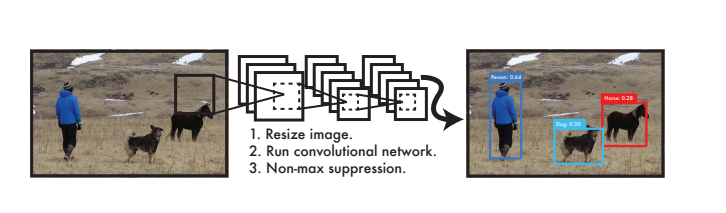
\includegraphics[scale=0.8]{pic/chap3/YOLO_total.jpg}
    \caption{YOLO目标检测系统}
    \label{fig:YOLO_total}
\end{figure}

\begin{enumerate}
    \item{YOLO非常快速。由于YOLO将目标检测问题简化为了回归问题,不再需要复杂的pipeline来进行特征提取和类别检测
    工作。}
    \item{与two-stage的目标检测算法不同,YOLO在预测时,使用了全局图像信息,因此能够显著降低错误率。}
    \item{由于YOLO端到端的训练特性,使得相比于R-CNN等检测算法,YOLO具有更强的可移植性。}
\end{enumerate}

YOLO使用整个图像的特征来预测每个目标的边界框(bounding boxes),可以同时预测所有类别的所有边界框。YOLO将输入图像
切分为S×S个网格,如果物体的中心落入某网格中,则该网格负责检测该物体。每个网格预测边界框和其置信度。边界框包括5个信息:
$x , y , w , h$和置信度。其中,$(x,y)$表示物体中心相对于网格单元框的坐标位置。$w,h$分别表示物体中心相对于整个
图像的宽度和高度。置信度则表示预测框和标注框的IOU(Intersection-Over-Union)值。模型逻辑如图\ref{fig:YOLO_model}所示。
每个网格预测$C$个条件概率,$Pr(Class_i|Object)$。
测试阶段,每个bounding box的置信度分数计算公式为:
\begin{equation}
    \centering
    \operatorname { Pr } \left( \text { Class } _ { i } | \text { Object } \right) * \operatorname { Pr } ( \text { Object } ) * \text { IOU } _ { \text { pred } } ^ { \text { truth } } = \operatorname { Pr } \left( \text { Class } _ { i } \right) * \text { IOU } _ { \text { pred } } ^ { \text { truth } }
    \label{YOLO_c}
\end{equation}

\begin{figure}[t]
    \centering
    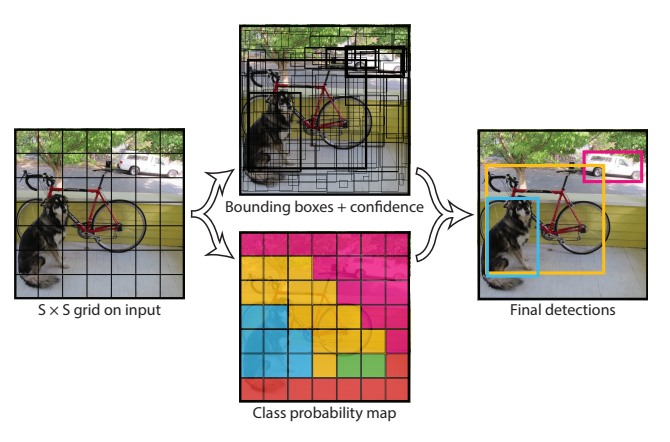
\includegraphics[scale=0.8]{pic/chap3/YOLO_model.jpg}
    \caption{YOLO模型逻辑}
    \label{fig:YOLO_model}
\end{figure}

\begin{figure} 
    \centering
    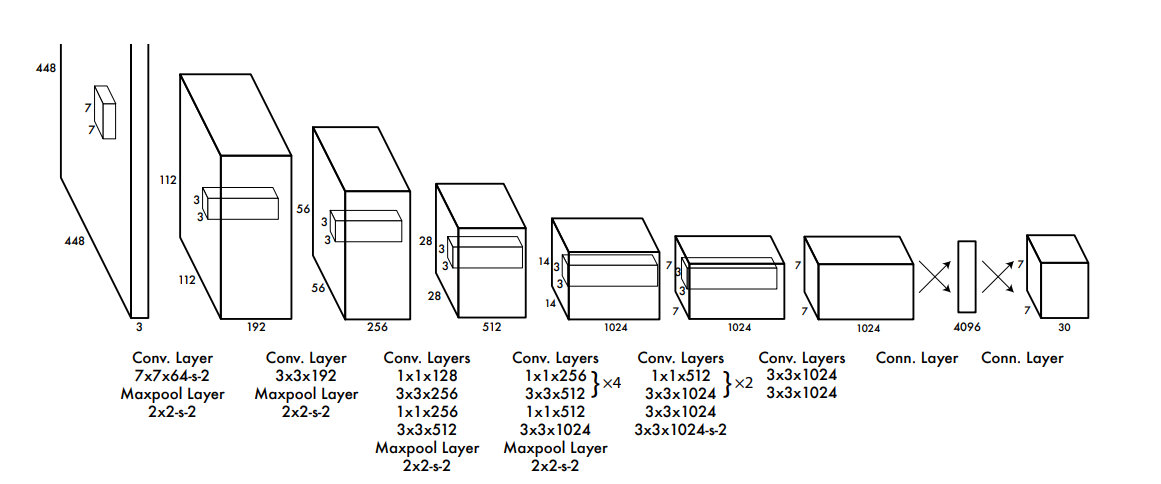
\includegraphics[scale=0.5]{pic/chap3/YOLO_construct.jpg}
    \caption{YOLO网络结构}
    \label{fig:YOLO_construct}
\end{figure}

在网络结构方面,YOLO使用卷积神经网络进行图片像素值到以上检测信息的映射。类似于GoogLeNet\cite{GoogLeNet2015},YOLO使用的网络结构为24层
卷积层后接两层全连接层。受Lin\cite{Lin}启发,YOLO将GoogLeNet初始模块中的3×3卷积层降维成1×1。整个网络结构如图\ref{fig:YOLO_construct}所示。


 
最后是模型的损失函数。由于目标检测需要预测目标物体的位置信息(即bounding box的信息)和类别信息,因此YOLO需要将两个任务的误差
损失结合到一个损失函数里面。YOLO采用sum-squared error的方式将bounding box的坐标误差和分类误差结合在一起。但如果两个任务的
损失权值一样,容易导致模型不稳定,不易收敛。因此采用对两个任务设置不同权重的方式。一方面,提高bounding box误差的权值,另一方面,
降低网格内部不包含物体中心的网格的分类损失权值。最终损失函数公式为:
$$\lambda _ { \text { coord } } \sum _ { i = 0 } ^ { S ^ { 2 } } \sum _ { j = 0 } ^ { B } 1 _ { i j } ^ { \mathrm { obj } } \left[ \left( x _ { i } - \hat { x } _ { i } \right) ^ { 2 } + \left( y _ { i } - \hat { y } _ { i } \right) ^ { 2 } \right]$$
$$+ \lambda _ { \text { coord } } \sum _ { i = 0 } ^ { S ^ { 2 } } \sum _ { j = 0 } ^ { B } 1 _ { i j } ^ { \mathrm { obj } } \left[ \left( \sqrt { w _ { i } } - \sqrt { \hat { w } _ { i } } \right) ^ { 2 } + \left( \sqrt { h _ { i } } - \sqrt { \hat { h } _ { i } } \right) ^ { 2 } \right]$$
$$+ \sum _ { i = 0 } ^ { S ^ { 2 } } \sum _ { j = 0 } ^ { B } 1 _ { i j } ^ { \mathrm { obj } } \left( C _ { i } - \hat { C } _ { i } \right) ^ { 2 }$$
$$+ \lambda _ { \mathrm { noobj } } \sum _ { i = 0 } ^ { S ^ { 2 } } \sum _ { j = 0 } ^ { B } 1 _ { i j } ^ { \mathrm { noobj } } \left( C _ { i } - \hat { C } _ { i } \right) ^ { 2 }$$
\begin{equation}
    \centering
    + \sum _ { i = 0 } ^ { S ^ { 2 } } 1 _ { i } ^ { \mathrm { obj } } \sum _ { c \in \text { classes } } \left( p _ { i } ( c ) - \hat { p } _ { i } ( c ) \right) ^ { 2 }
    \label{YOLO_J}
\end{equation}

其中,$1 _ { i } ^ { \mathrm { obj } }$表示网格$i$中是否存在物体的中心点; $1 _ { i j } ^ { \mathrm { obj } }$表示网格$i$预测的第$j$个
bounding box是否对该预测“负责”。$x , y , w , h$ 和 $C$的意义上文中已经进行了解释。
公式的前两行表示bounding box error,第一行表示网格中物体中心的坐标预测平方误差,第二行为宽度和高度预测的平方误差;第三、四行表示bounding box
的置信度损失,该损失分为网格内部是否落有物体中心分开计算。第五行代表分类误差。

总之,YOLO的思想,就是将目标检测问题通过设计合理的拟合对象和损失函数转换为回归问题。YOLO拟合的是图像像素值矩阵到bounding box和分类概率的映射
关系,通过最小化损失函数\ref{YOLO_J}得到最优的拟合关系。

\subsection{模型训练算法选择}

YOLO使用的网络结构为卷积神经网络,与通常的神经网络相同,其训练方法主要采用基于梯度下降的优化方法。
梯度下降法是优化领域最流行的算法,也是用于神经网络优化的最通用方法。它通过不断地
输入训练样本,朝着目标函数$J(\theta)$的负梯度的方向不断迭代网络参数$\theta \in \mathbb{R}^{d}$以优化
目标函数,逐步逼近最优参数解。学习率$\eta$表示每一步迭代的步长。

梯度下降法根据一次迭代使用多少数据可以分为
三个变种:批量梯度下降(Batch Gradient Descent,BGD)、随机梯度下降(Stochastic Gradient Descent,SGD)和
mini-batch梯度下降(mini-batch Gradient Descent,MBGD)。其中BGD使用所有数据进行一次迭代,SGD使用一个样本
进行一次迭代,MGD则介于两者之间,使用部分样本进行一次迭代。BGD的优点在于梯度计算准确,容易求得全局最优解,但需要消耗大量资源,并且
计算时内存不一定能加载所有数据;SGD使用的计算资源少,可以实现online-learning,但收敛速度慢。MBGD则是两者结合的产物。实际使用中,
一般使用MBGD。

然而,梯度下降法依然面临着许多问题,包括难以选取合适的学习率、避免陷入局部最优解等。为此,在梯度下降法的基础上,有许多算法
针对这些问题进行了优化。

\subsubsection{Momentum}
针对SGD在非凸优化问题中常见的“鞍点”问题,Momentum\cite{Momentum}可以帮助SGD在正确的方向上进行加速,而在不必要的方向上减少“震荡”。
Momentum通过将上一时刻更新矢量的$\gamma$倍添加到当前矢量上来实现:
$$v _ { t }  = \gamma v _ { t - 1 } + \eta \nabla _ { \theta } J ( \theta )$$
\begin{equation}
    \centering
    \theta  = \theta - v _ { t }
    \label{Momentum_F}
\end{equation}

\subsubsection{Adam}
Adaptive Moment Estimation(Adam)\cite{Adam}算法则是一个自适应学习率的梯度下降方法,它能够为每个网络参数自适应地
选择学习率。为了存储过去平方梯度的指数衰减平均值,Adam需要保存过去梯度$m_t$的指数衰减平均值:
$$m _ { t }  = \beta _ { 1 } m _ { t - 1 } + \left( 1 - \beta _ { 1 } \right) g _ { t }$$
\begin{equation}
    \centering
    v _ { t }  = \beta _ { 2 } v _ { t - 1 } + \left( 1 - \beta _ { 2 } \right) g _ { t } ^ { 2 } 
    \label{Adam_F_1}
\end{equation}

其中,$m_t$和$v_t$分别是梯度的第一时刻和第二时刻的估计值。同时,为了消除在初始时刻的偏差,通过如下公式更新$m_t$和$v_t$:
$$\hat { m } _ { t }  = \frac { m _ { t } } { 1 - \beta _ { 1 } ^ { t } } $$
\begin{equation}
    \centering
    \hat { v } _ { t }  = \frac { v _ { t } } { 1 - \beta _ { 2 } ^ { t } }
    \label{Adam_F_2}
\end{equation}
然后使用$m_t$和$v_t$来更新网络参数:
\begin{equation}
    \centering
    \theta _ { t + 1 } = \theta _ { t } - \frac { \eta } { \sqrt { \hat { v } _ { t } } + \epsilon } \hat { m } _ { t }
    \label{Adam_F_3}
\end{equation}

另外,与Adam类似的算法还有Adagrad\cite{Adagrad}、Adadelta\cite{adadelta}、RMSprop\cite{RMSprop}等算法,各个算法有各自的优势与劣势,下面一小节
中我们会对这些算法进行比较。

\subsubsection{优化算法比较与选择}
基于梯度下降法优化的各个算法,根据使用场景的不同,需要选择不同的算法。比如当输入数据比较稀疏时,使用自适应学习率的
方法不仅能取得最好的效果,同时也不需要调节学习率。总之,RMSprop是Adagrad的扩展,用以处理其急剧下降的学习率。它与Adadelta相同,
只不过Adadelta在更新规则中使用了参数更新的RMS。而Adam为RMSprop增加了偏差修正。RMSprop、Adadelta和Adam是非常相似的算法,
在类似的情况下表现良好。而随着梯度越来越稀疏,使用了偏差修正的Adam在训练的后期效果会更好。因此,Adam算法应该是大多数情况下
最优秀的训练算法。本课题在训练YOLOv3时使用的也是Adam算法。

\section{图像采集和数据获取}

任何模型,无论是深度学习模型还是传统的图像模型,第一步都是获取数据。数据是一切任务的前提,
只有有了数据,才能进行算法建模的下一步。因此,在训练深度学习目标检测模型之前,需要进行图像数据的
采集。这里使用ROS中的usb\_cam节点进行图像获取和数据采集。

由于我们使用的摄像头为USB摄像头,需要在ROS下安装USB驱动。安装之后,运行usb\_cam节点即可获取摄像头
的图像信息。由于训练模型需要的是图片数据,因此这里对usb\_cam节点源代码进行了更改,将实时视频的每一帧
图片保存到本地。同时,训练数据需要尽可能不同的图片,为了防止高FPS视频产生过多相同图片,这里将usb\_cam的
FPS从10降低到2,降低采样频率。更改方式为在usb\_cam.launch文件中加入如下配置:

$$ <param name="framerate" \quad value="2" />$$

同样为了降低图片的重复性,对视频图片进行随机降采样,即对每一帧图片,都以0.5的概率进行保存(或丢弃)。其具体公式
如下:

$$r = random(1)$$
\begin{equation}
    \centering
    IsSave =
        \begin{cases}
            1 & if \quad r >= 0.5\\
            0 & if \quad r < 0.5
        \end{cases}
\end{equation}

其中IsSave为usb\_cam节点的代码中的变量,当该变量为1时,将该帧图片保存到本地;否则对下一帧图片进行判断。

之后在摄像头固定的情况下,运行ROS的usb\_cam节点,将标注工件分别在摄像头下进行位置变换和角度变换等动作,从而
进行图片采集。采集的原则为,得到的图片集中要有单工件的不同位置和不同角度的图片,以及不同工件的共存图片。

\section{数据标注}

基于深度学习的目标检测模型属于监督学习,监督学习需要大量的有标注样本作为Ground Truth,通过标注样本计算损失函数的梯度,
然后使用Adam优化算法更新网络参数,直到损失函数得到最小值,网络得到最优解。因此,上一小节采集得到的图片需要进行标注。由于
YOLO模型是拟合图像像素矩阵值到bounding box和分类概率的映射关系,因此我们需要标注每张图像中工件的bounding box值,包括$x , y , w , h$,
以及该工件所属的类别。每张图片需要五个值。

\begin{figure}[h]
    \begin{minipage}{0.5\linewidth}
        \centering
        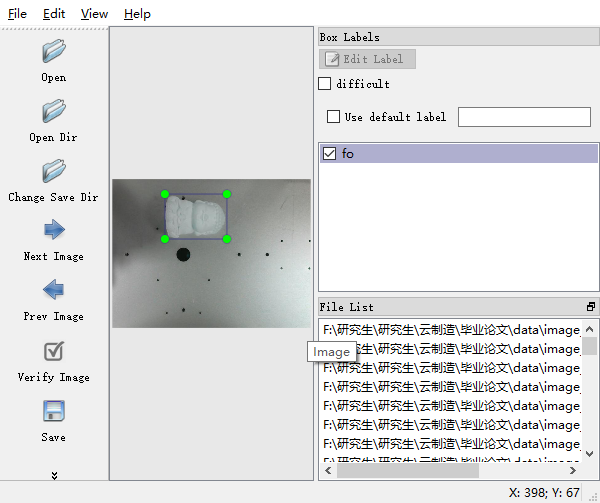
\includegraphics[scale=0.5]{pic/chap3/labelimg.jpg}
        \caption{LabelImg标注界面}
        \label{fig:LabelImg}
    \end{minipage}
    \begin{minipage}{0.5\linewidth}
        \centering
        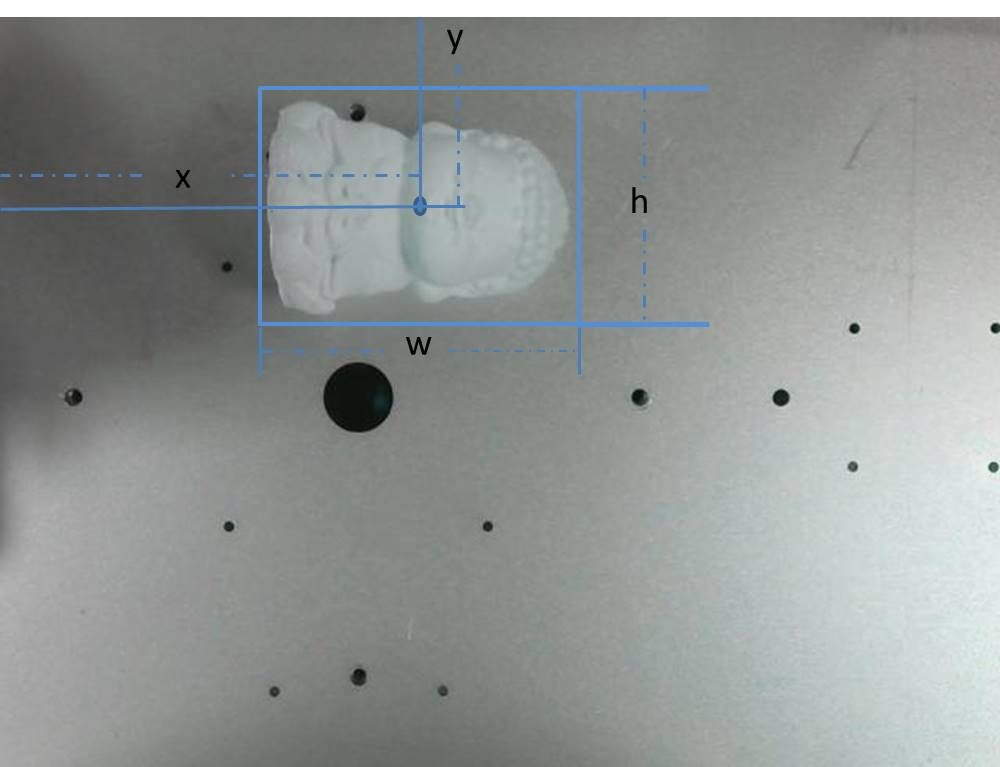
\includegraphics[scale=0.5]{pic/chap3/标注信息图示.jpg}
        \caption{标注信息图示}
        \label{fig:labelimg_info}
    \end{minipage}
\end{figure}

我们使用标注工具LabelImg \cite{LabelImg} 对采集到的图片数据进行标注,LabelImg标注界面如图 \ref{fig:LabelImg} 所示。每张图片标注并保存后会
生成一个与图片同名的txt文件,该文件内容如下(以其中一张图片为例):
$$1 \quad 0.420312 \quad 0.251042 \quad 0.312500 \quad 0.302083$$
该文件中一共5个值,分别代表物体的类别,$x , y , w , h$,其意义如表 \ref{table:LabelImg:info} 所示。在图片上的含义见图 \ref{fig:labelimg_info}。
{
    \begin{table}[htb]
        \zihao{5}
        \caption{标注数据含义}
        \label{table:LabelImg:info}
        \centering
        \begin{tabular}[t]{p{0.15\columnwidth} | p{0.15\columnwidth} | p{0.15\columnwidth} | p{0.15\columnwidth} | p{0.15\columnwidth}}
            \hline
            工件所属类别所占编号 & 工件中心横坐标x占整张图片宽度的比例 & 工件中心纵坐标y占整张图片高度的比例 & 边界框宽度w占整张图片宽度的比例 & 边界框高度h占整张图片的比例 \\
            \hline
            1 & 0.420312 & 0.251042 & 0.312500 & 0.302083\\
            \hline
        \end{tabular}
    \end{table}
}

最终共标注图片213张,产生213个txt文件。一共416个文件,构成了训练模型的标注数据集。将这些文件随机打乱之后,随机选取90\%作为训练数据集,剩下
10\%为测试数据集。

\section{目标检测模型训练与评估}
YOLO模型采用的网络结构为卷积神经网络,训练方法为基于梯度下降法的自适应学习率训练算法Adam。由于数据集图片数量不多,因此采用迁移学习的
方法来进行训练。此外,由于Jetson TX2计算能力有限以及需要检测的工件数量不多、特征明显,因此需要将YOLOv3的模型进行精简,以保证YOLOv3模型
部署在Jetson TX2上依然能够有足够的性能表现。

\subsection{模型评估方法}

首先介绍模型的评估方法。合理的评估方法能帮助我们合理的选择出最优的模型,从而取得最优的效果。

目标检测领域的评价体系中,最常用的评价指标为IOU(Intersection-Over-Union),同时,该参数也参与了Yolo损失函数的计算。因此,
本文选用IOU值作为评价模型的指标。

IOU即模型产生的目标窗口和标记窗口的重叠率。其公式如下:

\begin{equation}
    \centering
    I O U = \frac { \text { DetectionResult } \cap \text {GroundTruth} } { \text {DetectionResult} \cup \text {GroundTruth } }
    \label{IOU_equation}
\end{equation}

如图 \ref{fig:IOU_equation},IOU即图中蓝色区域面积除以所有图形面积之和。

\begin{figure}[htbp]
    \centering
    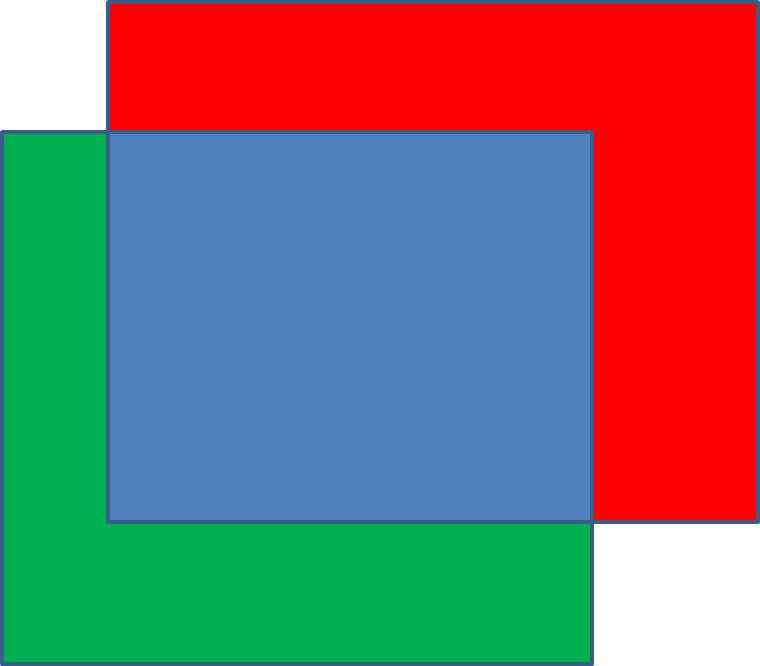
\includegraphics[scale=0.8]{pic/chap3/IOU.jpg}
    \caption{IOU计算方式图例}
    \label{fig:IOU_equation}
\end{figure}

\subsection{迁移学习}
机器学习是人工智能的重要方法。机器学习解决的是让机器自主地从数据中获取知识,从而应用于新的问题。而迁移学习作为机器学习的
一个重要分支,侧重于将已经学习过的知识迁移应用于新的问题。迁移学习的核心问题是如何找到新问题和原问题的相似性,只有找到
了相似性,才能将原问题学习到的知识应用到新问题上。使用机器学习的语言来说,迁移学习,是指利用数据、任务或模型之间的相似性,
将在旧领域学习过的模型,应用于新领域的一种学习过程。

迁移学习的研究主要是为了解决以下问题 \cite{TL_tutorial}:
 
\begin{enumerate}
    \item {大数据与少标注之间的矛盾。
    
    深度学习模型具有海量的参数需要训练,而这些训练都依赖于大量的标注数据。若标注
    数据过少,复杂的深度学习模型很容易陷入过拟合,而得不到好的训练结果。然而数据的标注
    是一个耗时且昂贵的操作,因此深度学习需要大量标注数据与数据标注的困难形成了一个矛盾。
    通过寻找与目标数据相近的有标注数据,利用这些数据来构建模型,增加目标数据的标注。迁移
    数据标注的方式可以有效解决这种问题。}
    \item {大数据与弱计算之间的矛盾。
    
    深度学习模型一般需要海量的计算资源,如NLP界的巨无霸模型BERT\cite{BERT}模型,谷歌
    使用了16个TPU集群(共64块TPU)训练了四天。而大部分开发者是无法触及这么大规模的计算资源
    的。利用迁移学习的思想,我们可以使用那些已经在大数据上训练好的模型,迁移到自己的任务中,
    针对自己的任务进行微调,从而获得更好的模型效果。}
\end{enumerate}

\begin{figure}[htbp]
    \centering
    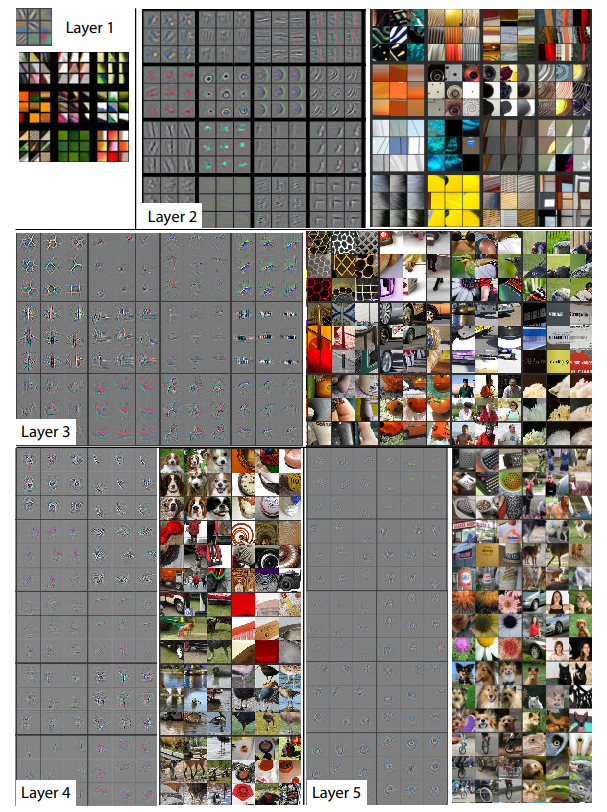
\includegraphics{pic/chap3/imagenet_vis.jpg}
    \caption{卷积神经网络中间层特征可视化}
    \label{fig:ImageNet:vis}
\end{figure}
 
表 \ref{table:TL:biyao} 展示了迁移学习的必要性。
{
    \begin{table}[htb] 
        \zihao{5}
        \caption{迁移学习的必要性}
        \label{table:TL:biyao}
        \centering
        \begin{tabular}[t]{c|c|c}
            \hline
            矛盾 & 传统机器学习 & 迁移学习 \\
            \hline
            大数据与少标注 & 增加人工标注,耗时且昂贵 & 数据的迁移标注\\
            \hline
            大数据与弱计算 & 只能依赖强大的计算能力 & 模型迁移\\
            \hline
        \end{tabular}
    \end{table}
}

在图像领域,通常作为迁移学习的基模型的为Google在ImageNet数据集上预训练的模型。ImageNet
是目前世界上图像识别最大的数据库。在ImageNet上训练得到的神经网络模型,其中间层一般都具有
表征图像底层或高层特征的能力。如图 \cite{ImageNet_vis} \ref{fig:ImageNet:vis} ,在ImageNet上训练得到卷积神经网络,其底层抽取出
边缘角点以及颜色特征,越到高层越呈现出具体的特征。由于预训练得到的网络参数,已经具备了表征图像特征的能力,因此
从这些网络参数出发,在特定的图像任务上,已经比较接近最优解,只需要在特定任务的小数据集上进行再次训练,即可
达到该任务下的最优解。



在本文中,将选用在ImageNet预训练的YOLO模型作为迁移学习的基模型,即使用在大数据集上预训练得到的网络
参数作为本任务的网络初始参数,然后使用本任务的数据集上继续迭代参数,直到网络收敛。






\subsection{模型训练与选择}
结合自动分拣系统的硬件实际情况,本课题一共训练了两种YOLOv3模型,两种模型除网络配置外,其余所有情况包括
数据集、训练方法等均相同。第一种使用论文作者的原始配置,称为YOLOv3,另一种则将网络结构进行了精简,使用了更少
的网络参数,叫做YOLOv3-tiny。表 \ref{table:model:config} 展示了两种模型配置的不同之处。

{
    \begin{table}[htb] 
        \zihao{5}
        \caption{YOLOv3和YOLOv3-tiny配置参数比较}
        \label{table:model:config}
        \centering
        \begin{tabular}[t]{c|c|c|c|c|cc|c|c|c}
            \hline
            配置 & batch & width & height & 卷积层数 & 池化层数  \\
            \hline
            YOLOv3 & 16 & 640 & 480 & 75 & 0 \\
            \hline
            YOLOv3-tiny & 16 & 640 & 480 & 13 & 6 \\
            \hline
            配置 & shortcut(Res)层数 & unsample层数 & Route层数 & yolo层数\\
            \hline
            YOLOv3 & 23 & 2 & 4 & 3\\
            \hline
            YOLOv3-tiny & 0 & 1 & 2 & 2\\
            \hline
        \end{tabular}
    \end{table}
}

其中,batch为训练过程中每迭代一次参数使用的样本数量;width和height为所使用的训练图片的宽度和高度;卷积层数为神经网络结构中,卷积层
的数量;池化层数为网络中使用的最大池化层(max-pooling)的数量;shortcut层类似于ResNet \cite{ResNet}中的残差连接,用于将底层特征传输到高层;
upsample层的作用是对前一层的特征进行上采样;Route层用于索引特征图;yolo层为检测层。

使用的迁移学习基模型也是基于上述两种配置在ImageNet上预训练得到的网络参数。使用YOLO的开源训练框架DarkNet \cite{DarkNet}
进行训练。训练过程中的参数情况如图 \ref{fig:train:log} 所示。
\begin{figure}[h]
    \centering
    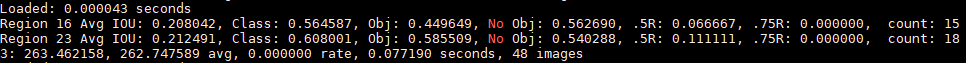
\includegraphics[width=\textwidth]{pic/chap3/train_log.png}
    \caption{训练过程参数示意图}
    \label{fig:train:log}
\end{figure}

\begin{figure}[t]
    \centering
    \subfigure[Loss曲线图 Batch:0-2000]{
        \label{fig:Loss:fullbatch}
        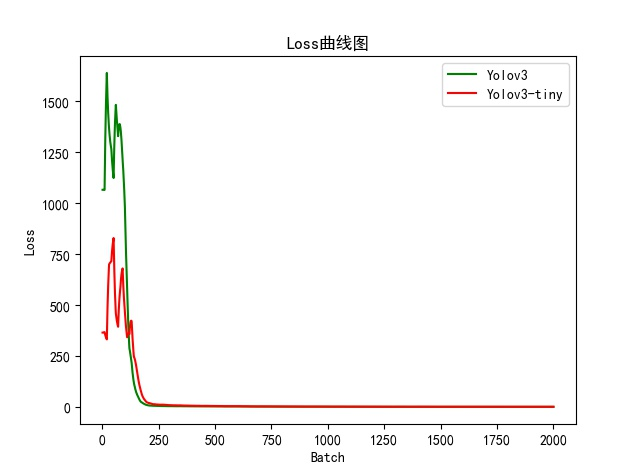
\includegraphics[width=0.46\columnwidth]{pic/chap3/Loss-v3&v3_tiny.jpeg}
    }
    \subfigure[Loss曲线图 Batch:500-2000]{
        \label{fig:Loss:partbatch}
        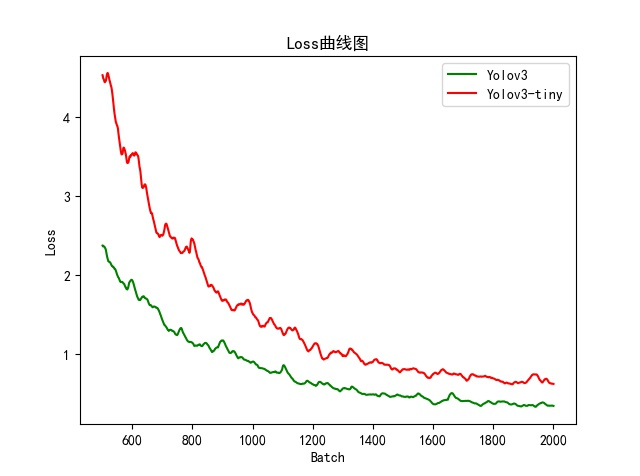
\includegraphics[width=0.46\columnwidth]{pic/chap3/Loss-v3&v3_tiny-scaled.jpeg}
    }
    \caption{Yolov3和Yolov3-tiny的Loss曲线对比图}
    \label{fig:Loss}
\end{figure}

\begin{figure}[t]
    \centering
    \subfigure[IOU曲线图 Batch:0-2000]{
        \label{fig:IOU:fullbatch}
        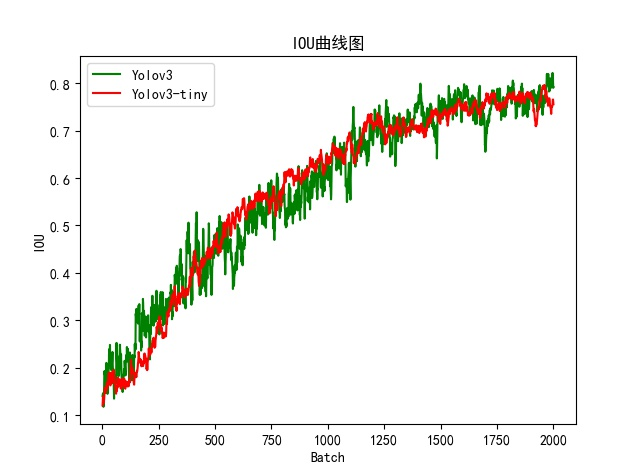
\includegraphics[width=0.46\columnwidth]{pic/chap3/IOU-v3&v3_tiny.jpeg}
    }
    \subfigure[IOU曲线图 Batch:500-2000]{
        \label{fig:IOU:partbatch}
        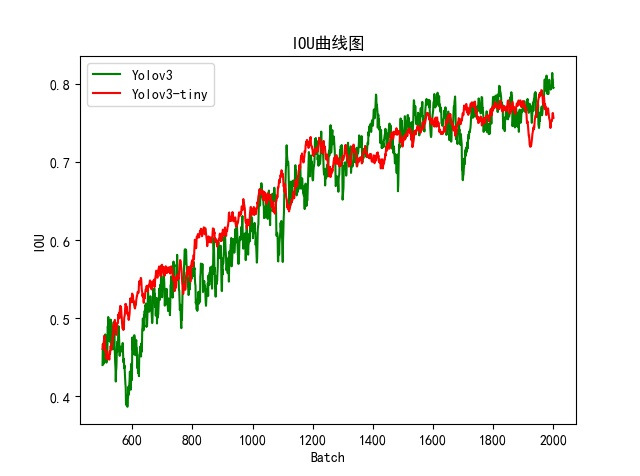
\includegraphics[width=0.46\columnwidth]{pic/chap3/IOU-v3&v3_tiny-scaled.jpeg}
    }
    \caption{Yolov3和Yolov3-tiny的IOU曲线对比图}
    \label{fig:IOU}
\end{figure}

图 \ref{fig:train:log} 显示了所有训练图片的一个批次(batch)。图片的第一行表示该批次训练所用时间。剩下的输出包括批输出
和分块输出。该图的批输出如下:
$$3: \quad 263.462158,\quad 262.747589 \; avg,\quad  0.000000 \; rate, \quad 0.077190 \; seconds, \quad 48 \; images$$

其中3表示当前训练的迭代次数;263.462158代表总体的Loss;262.747589 avg表示平均Loss,越低越好;
0.000000 rate表示当前的学习率;0.077190 seconds表示当前批次花费的总时间;48 images表示到目前为止训练的图片的总数量。

\begin{figure}[h]
    \centering
    \subfigure[Loss曲线图 Batch:0-2000]{
        \label{fig:Loss-TL:fullbatch}
        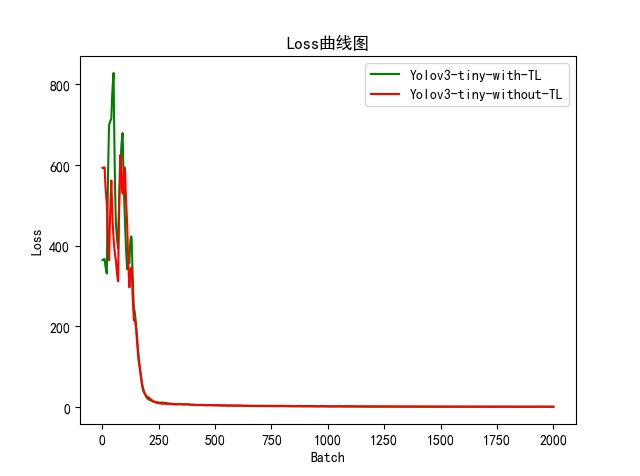
\includegraphics[width=0.46\columnwidth]{pic/chap3/Loss-v3_tiny&v3_tiny_noTL.jpeg}
    }
    \subfigure[Loss曲线图 Batch:500-2000]{
        \label{fig:Loss-TL:partbatch}
        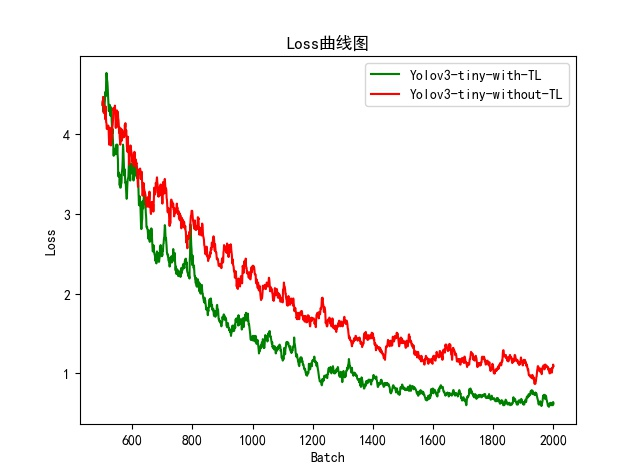
\includegraphics[width=0.46\columnwidth]{pic/chap3/Loss-v3_tiny&v3_tiny_noTL-scaled.jpeg}
    }
    \caption{Yolov3-tiny是否使用迁移学习的Loss曲线对比图}
    \label{fig:Loss_TL}
\end{figure}


\begin{figure}[h]
    \centering
    \subfigure[IOU曲线图 Batch:0-2000]{
        \label{fig:IOU-TL:fullbatch}
        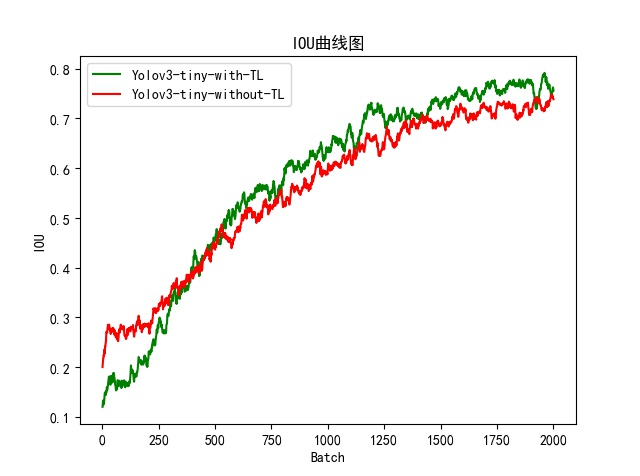
\includegraphics[width=0.46\columnwidth]{pic/chap3/IOU-v3_tiny&v3_tiny_noTL.jpeg}
    }
    \subfigure[IOU曲线图 Batch:500-2000]{
        \label{fig:IOU-TL:partbatch}
        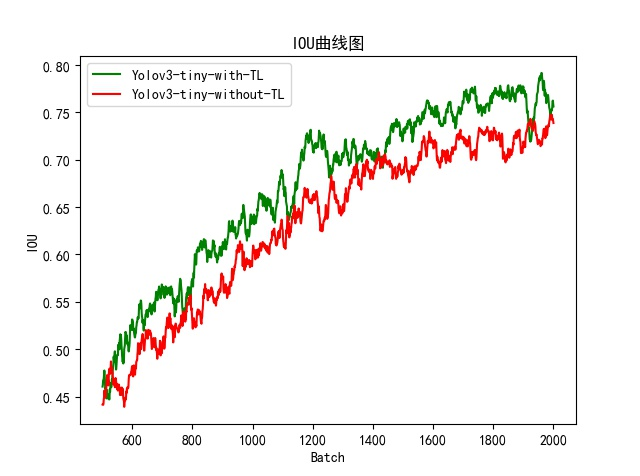
\includegraphics[width=0.46\columnwidth]{pic/chap3/IOU-v3_tiny&v3_tiny_noTL-scaled.jpeg}
    }
    \caption{Yolov3-tiny是否使用迁移学习的IOU曲线对比图}
    \label{fig:IOU_TL}
\end{figure}

该图的分块输出如下:
$$Region\;23 \quad Avg IOU: 0.212491, \  Class: 0.608001, \  Obj: 0.585509, \  No Obj: 0.540288, $$
$$\ .5R: 0.111111, \ .75R: 0.000000, \  count: 18$$

上述参数中,Region 23 Avg IOU表示在当前分区内,图片的平均IOU,表示预测的矩形框和真实目标框的交集与并集之比。这里是21.25\%;Class:0.608001表示标注物体
的分类正确率,该值趋近于1;Obj: 0.585509表示把正样本判断为正样本的平均置信度为0.59,该值期望趋近于1;No Obj则期望趋近于0;.5R和.75R分表表示当前模型
在所有分块中检测出的正样本数量与实际的正样本数量的比值,全部样本被检测到这两个值均为1;count则表示所有分块的图片中
包含正样本的图片的数量。

训练过程中,在达到不同的batch数节点时会进行权重的保存。具体来说,前1,000个batch,每100个batch会进行一次权重的保存;之后每10,000个batch进行一次权重
文件保存。当平均损失降低到0.2以下时即可结束训练。最后选择平均IOU最高的权重文件作为最终使用的网络参数。


\begin{figure}[t]
    \centering
    \subfigure[预测用时曲线图]{
        \label{fig:inf_time:curve}
        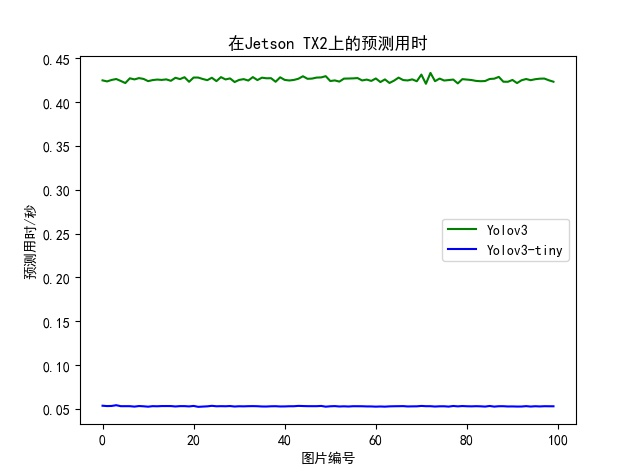
\includegraphics[width=0.46\columnwidth]{pic/chap3/time-v3&v3_tiny.jpeg}
    }
    \subfigure[预测平均用时柱状图]{
        \label{fig:inf_time:bar}
        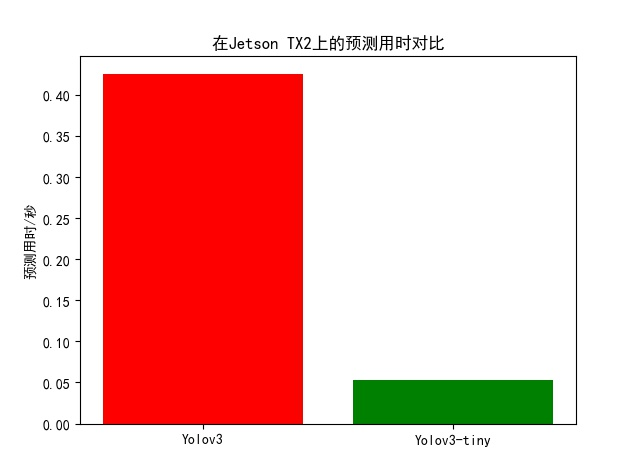
\includegraphics[width=0.46\columnwidth]{pic/chap3/time-v3&v3_tiny-avg.jpeg}
    }
    \caption{Yolov3和Yolov3-tiny的预测用时对比}
    \label{fig:inf_time}
\end{figure}

\begin{figure}[t]
    \centering
    \subfigure[模型预测效果1]{
        \label{fig:model_pre:1}
        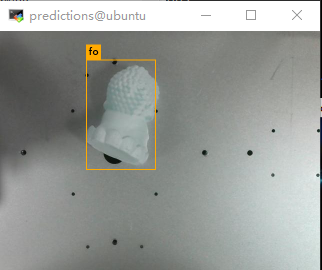
\includegraphics[width=0.46\columnwidth]{pic/chap3/model_prediction_1.png}
    }
    \subfigure[模型预测效果2]{
        \label{fig:model_pre:bar}
        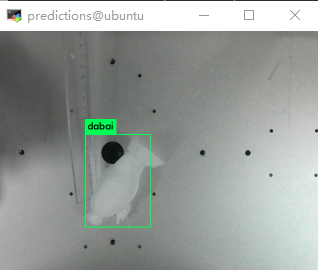
\includegraphics[width=0.46\columnwidth]{pic/chap3/model_prediction_2.png}
    }
    \caption{模型预测效果示意图}
    \label{fig:model_pre}
\end{figure}


Yolov3和Yolov-tiny模型训练过程的Loss变化曲线如图 \ref{fig:Loss} 所示。整体来看,经过2000个Batch,两个模型收敛的速度
及达到的损失函数值非常接近。Yolov3最终的Loss值略低于Yolov3-tiny。两个模型训练过程中的IOU变化曲线如图 \ref{fig:IOU} 所示。
两个模型的IOU变化及最终达到的IOU值相似。由上述两幅图可知,针对该任务,Yolov3-tiny和Yolov3的效果表现类似。而两者在Jetson TX2进行
模型预测的用时情况如图 \ref{fig:inf_time} 所示,由图可知,Yolov3-tiny在Jetson TX2上的预测用时远远小于Yolov3,说明了本任务选用Yolov3-tiny模型配置
的优势。

同时,在基于ImageNet预训练模型训练之外,本文也训练了不使用迁移学习的模型,以论证迁移学习的必要性和有效性。如图 \ref{fig:Loss_TL},是否使用迁移学习
模型的训练过程Loss曲线对比显示,使用迁移学习的Yolov3-tiny模型,在经过2000个Batch的训练后,取得了比不使用迁移学习的Yolov3-tiny模型更低
的Loss值。IOU方面,如图 \ref{fig:IOU_TL},IOU对比曲线显示,使用迁移学习的Yolov3-tiny模型,取得了更高的IOU值。这两幅图充分说明了基于本任务
选用基于ImageNet预训练的模型进行迁移学习的必要性。

通过对比,本论文最终选用基于迁移学习的Yolov3-tiny模型,作为自动分拣系统的目标检测算法进行使用。模型预测效果如图 \ref{fig:model_pre} 所示。
由图可知,模型可以准确的预测出目标物体的边框和类别。

\section{目标检测模型部署}

目标检测模型训练好之后,只能用于测试图片文件查看效果,并不能实际应用。因此,需要将训练好的Yolo目标检测模型进行封装,
将其作为一个ROS节点,加入自动分拣系统的ROS通信网络,以便被其他模块调用。

本文使用darknet\_ros \cite{darknet_ros}对模型进行封装。将darknet\_ros配置到Jetson TX2上之后进行编译,然后根据
本任务进行配置。主要包括模型权重文件和配置文件替换、ROS相关配置和启动项配置。配置好之后,启动yolov3.launch节点,
即可使用之前训练好的模型进行检测,并将边框和类别信息发布到/darknet\_ros/boundingboxes话题下,其余模块可通过订阅
该话题来接收物体的类别和边框信息。

\section{本章小结}
本章主要介绍图形处理模块。本文的自动分拣系统使用了传统的图像算法和基于深度学习的目标检测算法,本章介绍了所使用
的算法的原理。然后介绍了得到目标检测算法模型的流程,包括数据获取、数据标注、模型的训练和评估方法。然后选择了
使用迁移学习的Yolov3-tiny配置模型进行实际应用。最后介绍了如何将训练好的模型部署到ROS的通信节点中。